\documentclass[14pt]{beamer}
\usetheme{Dresden}
\usepackage[utf8]{inputenc}
\usepackage[russian]{babel}
\usepackage[OT1]{fontenc}
\usepackage{amsmath}
\usepackage{amsfonts}
\usepackage{amssymb}
\usepackage{graphicx}
\usepackage{wrapfig}
\usepackage{float}
\frenchspacing
\usepackage{listings}
\title{Семейство операционных систем Linux}
\author{Давиденко Алексей}

\usecolortheme[dark,accent=green]{solarized}
\setbeamercovered{transparent}
\setbeamertemplate{navigation symbols}{} 
\date{}
\begin{document}

\begin{frame}[plain]
\titlepage
\end{frame}

\begin{frame}
\begin{block}{Linux"---}
\textit{Семейство Unix-подобных операционных систем
на базе ядра Linux}
\end{block}
\end{frame}

\begin{frame}
\begin{block}

\textbf{Linux} является третьей по популярности 
операционной системой на сегодняшний день.\\
Отчасти, это связанно с тем, что Linux-системы 
распространяются бесплатно в основном в виде 
различных дистрбутивов.
\end{block}
\end{frame}

\begin{frame}
\begin{block}

Считается, что Linux имеет двух прародителией, на 
основании которых он и возник:
\\операционная система \textbf{UNIX} и проект 
\textbf{GNU}
\end{block}
\end{frame}

\begin{frame}
\begin{block}

\centering
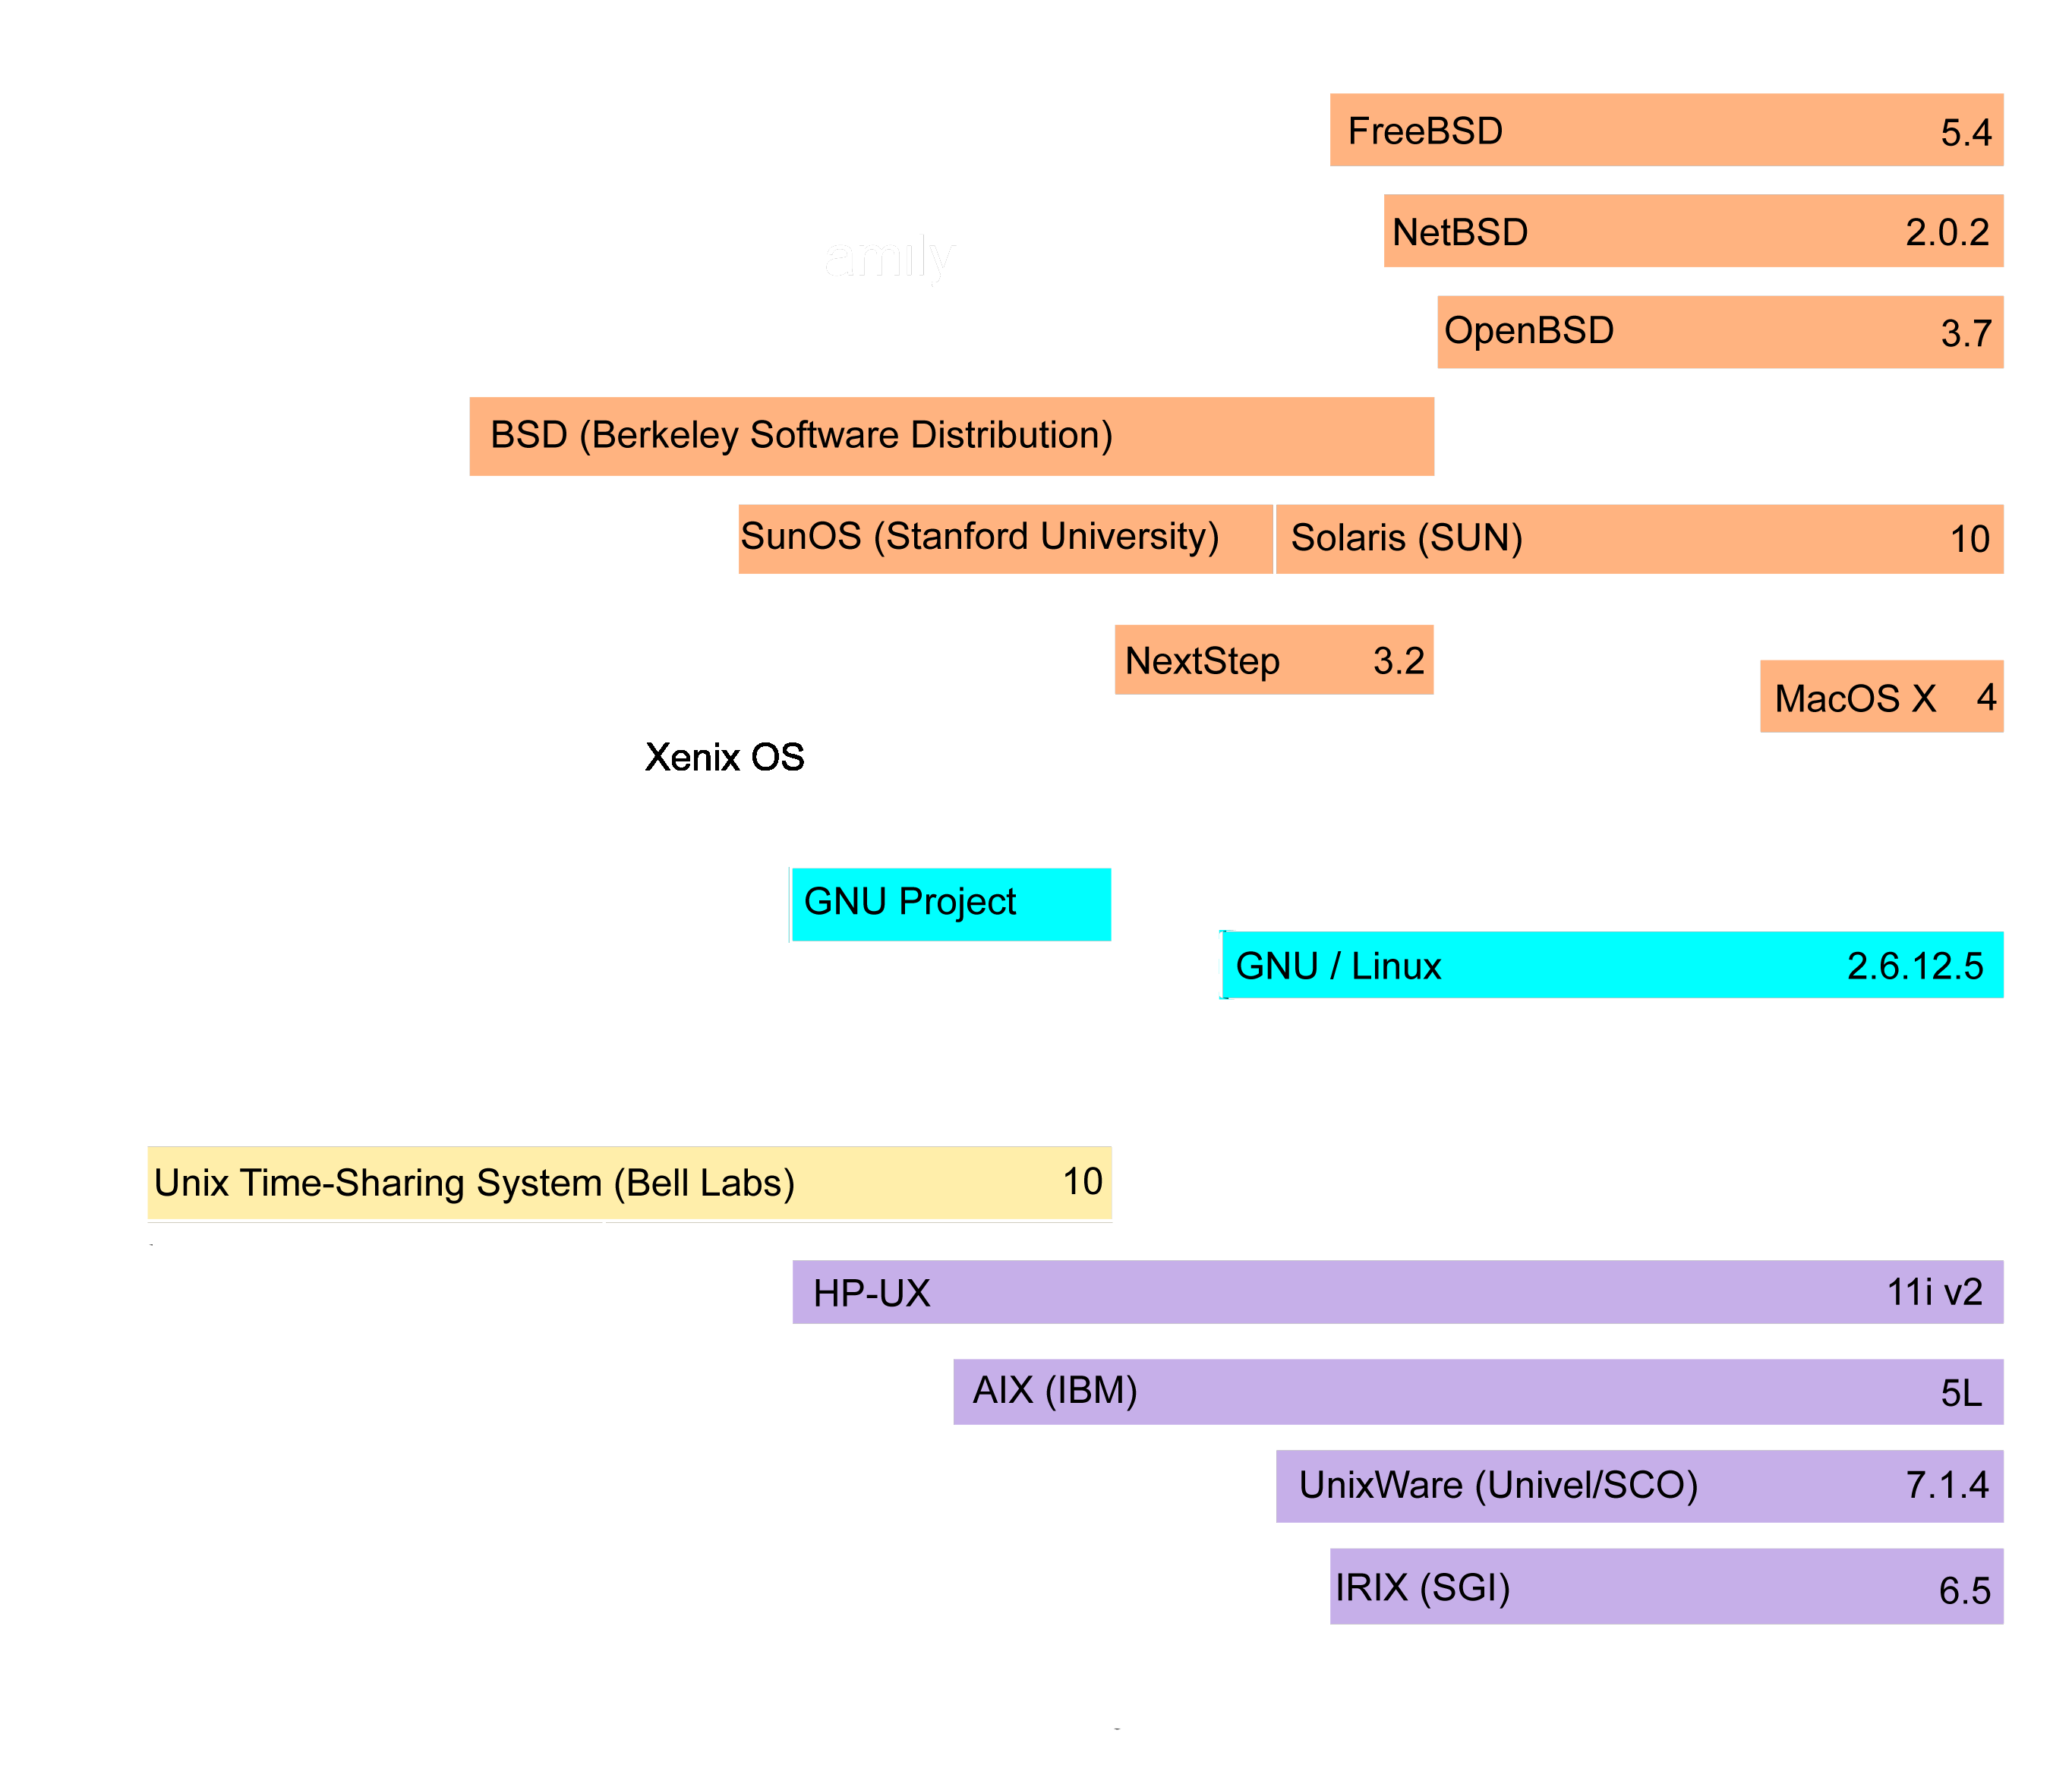
\includegraphics[height=0.92\textheight]
{Timeline_of_Unix_families.png}
\end{block}
\end{frame}

\begin{frame}
\begin{block}{История создания}
\par Для подключения к сети университета создатель 
Linux, \textsl{Линус Бенедикт Торвальдс}, установил 
на своё домашний компьютер \textbf{OC Minix}, 
который в последствие переписал терминал и файлувую 
систему операционной системы.
\par Так как из попытки написания терминала 
появился скелет новой операционной системы, Линус 
начал разработку собственной системы.
\end{block}
\end{frame}

\begin{frame}
\begin{block}

\textsl{25 августа 1991} года Торвальдс написал e-
mail в список рассылки пользователей Minix, в 
котором сообщал, что занимается разработкой 
операционной системы и 

просил указать пожелания и предложения от 
пользователей Minix. Этот день считается днём 
рождения 
Linux. А \textsl{5 октября} он выпустил  версию  
ядра  0.2  и  выложил  исходные  коды  в  интернет.  
Многие
заинтересовались этой системой.

\end{block}
\end{frame}

\begin{frame}
\begin{block}

Первые дистрибутивы Linux появились вскоре после 
того, как Линус Торвальдс выпустил разработанное им 
ядро под лицензией \textsl{GPL}. Отдельные 
программисты (и группы программистов) начали 
разрабатывать как программы инсталляции, так и 
другие прикладные программы, пользовательский 
интерфейс, программы управления 
пакетами и выпускать свои дистрибутивы.

\end{block}
\end{frame}

\begin{frame}[shrink=10]
\begin{block}

После выпуска версии 1.0, ядро продолжило свое 
развитие в виде двух веток - \underline{стабильной} 
(рекомендуемой к широкому использованию) и 
\underline{экспериментальной} (тестовая версия, 
включающее новые возможности и активно 
разрабатываемое). Стабильные версии имели чётную 
вторую цифру в номере (например 1.0.1), а 
экспериментальные нечётную (например 1.1.4). После 
того как экспериментальная версия была достаточно 
обработана и годилась к использованию широкими 
слоями пользователей, её второй номер увеличивался 
на единицу и она считалась стабильной. Одновременно 
с этим появилась новая экспериментальная версия.

\end{block}
\end{frame}

\begin{frame}
\begin{block}

\textsl{В 1996 году} был выбран символ системы. Им 
стал добродушный и в меру упитанный пингвинёнок 
\textbf{Такс}, отличительная особенность которого - 
жёлтые лапы и клюв.

\centering

\includegraphics[scale=0.35]{Tux.png}
\end{block}
\end{frame}

\begin{frame}[shrink=10]
\begin{block}

Широкое распространение операционной системы Linux 
началось со времени выхода стабильной версии ядра 
версии 2.2 в январе 1999 года. На нее обратили 
внимание производители серверных приложений, баз 
данных, Web-серверов, а также приложений для 
всякого рода защиты ПК. Произошло это во многом 
благодаря широкому распространению веб-сервера 
Apache. На сегодняшний день порядка 65\% web-
серверов работают на ОС Linux, Linux используется 
на 91 \% самых мощных суперкомпьютеров планеты и на 
подавляющее большинстве компьютеров обслуживающих 
систему доменных имён DNS. Инфраструктура самой 
популярной поисковой системы Google.com и сайта 
wikipedia.org, строится на базе множества серверов 
с Linux.
\end{block}
\end{frame}

\begin{frame}[shrink=10]
\begin{block}

Благодаря изменениям последних лет, число 
инсталляций Linux всё время растёт. Ясно что эта 
система имеет большое будущее. В компьютерных 
магазинах, зачатую, помимо Windows, можно увидеть 
Linux как предустановленную систему. В России идёт 
процесс внедрения Linux и свободного программного 
обеспечения в школах и государственных учреждениях.
\end{block}
\end{frame}

\begin{frame}[shrink=10]
\begin{block}

То, что зарождалось как программа для подключения к 
университетскому компьютеру, превратилось в самый 
грандиозный проект мира свободного программного 
обеспечения. Сегодня по данным Евросоюза, стоимость 
разработки ядра Linux с нуля при коммерческом 
подходе, составляет более одного миллиарда евро. 
Модель коллективной разработки СПО доказала свою 
жизнеспособность. Для многих оказалось открытием, 
возможность достойной конкуренции разработки кучки 
энтузиастов против продуктов транснациональных 
корпораций с многомиллиардными оборотами. Linux в 
очередной раз, доказал, что деньги в этом мире не 
главное, и добрая воля человека способна на великие 
свершения.

\end{block}
\end{frame}

\begin{frame}[shrink=10]
\begin{block}{Список использованных источников}
\begin{thebibliography}{99}
	\bibitem{Ione} Костромина В.А. "Свободная 
	система для свободных 
	людей", 2005г.
	
	\bibitem{Itwo} Федорчук Алексей "Linux: 
	предыстория в тезисах", 
	2006г.
	
	\bibitem{Ithree} Статьи с сайта
	http://ru.wikipedia.org
	
	\bibitem{Ifour} Далхаймер М., Уэлш М. 
	"Запускаем Linux" \,, 2008г., 
	Символ-Плюс.
	
	\bibitem{Ifive} Маянк Шарма. Рождение ядра 
	Linux, 2016г.,~—
	~Октябрь~(\textnumero 10 (215)). — С. 24-31.
\end{thebibliography}
\end{block}
\end{frame}

\begin{frame}[plain]
\vfill
\centering
\begin{Huge}
Спасибо~за~внимание!
\end{Huge}
\vfill

\end{frame}

\end{document}
